\chapter{Conclusions}

\section{Conclusions}

In this work, we introduced a method that leverages self-supervised deep neural networks to learn low-dimensional music latent representations with applications to music boundary detection. Building on existing approaches and architectures, we replaced traditional features with deep embeddings trained to represent high-level musical information to analyze its performance in music segmentation tasks.

While not outperforming state-of-the-art existing baselines and in contrast to similar research findings such \cite{deepfeaturesegment, SalamonDeepSegmentation}, our musically-informed technique has significant potential for boundary detection tasks given its overall performance improvement alongside the training set enlargement. Most likely, so does for nearly all MIR downstream tasks that are not purely sonic-based.

The questions of whether such general-purpose audio representation can mimic human hearing \cite{Li2023MERT:Training, Turian2022HEAR:Representations} or whether these do decode underlying high-level musical content effectively remain scientifically unanswered given the lack of evaluation in that regard. That is a "thorn in our side" that we will pursue.

\section{Discussion}

While whether our model decodes underlying high-level musical content effectively remains scientifically unanswered, the outstanding performance in precision metric

Too little representation layer?

Too little model for raw audio input? \cite{verydeep}

\begin{figure}
    \centering
    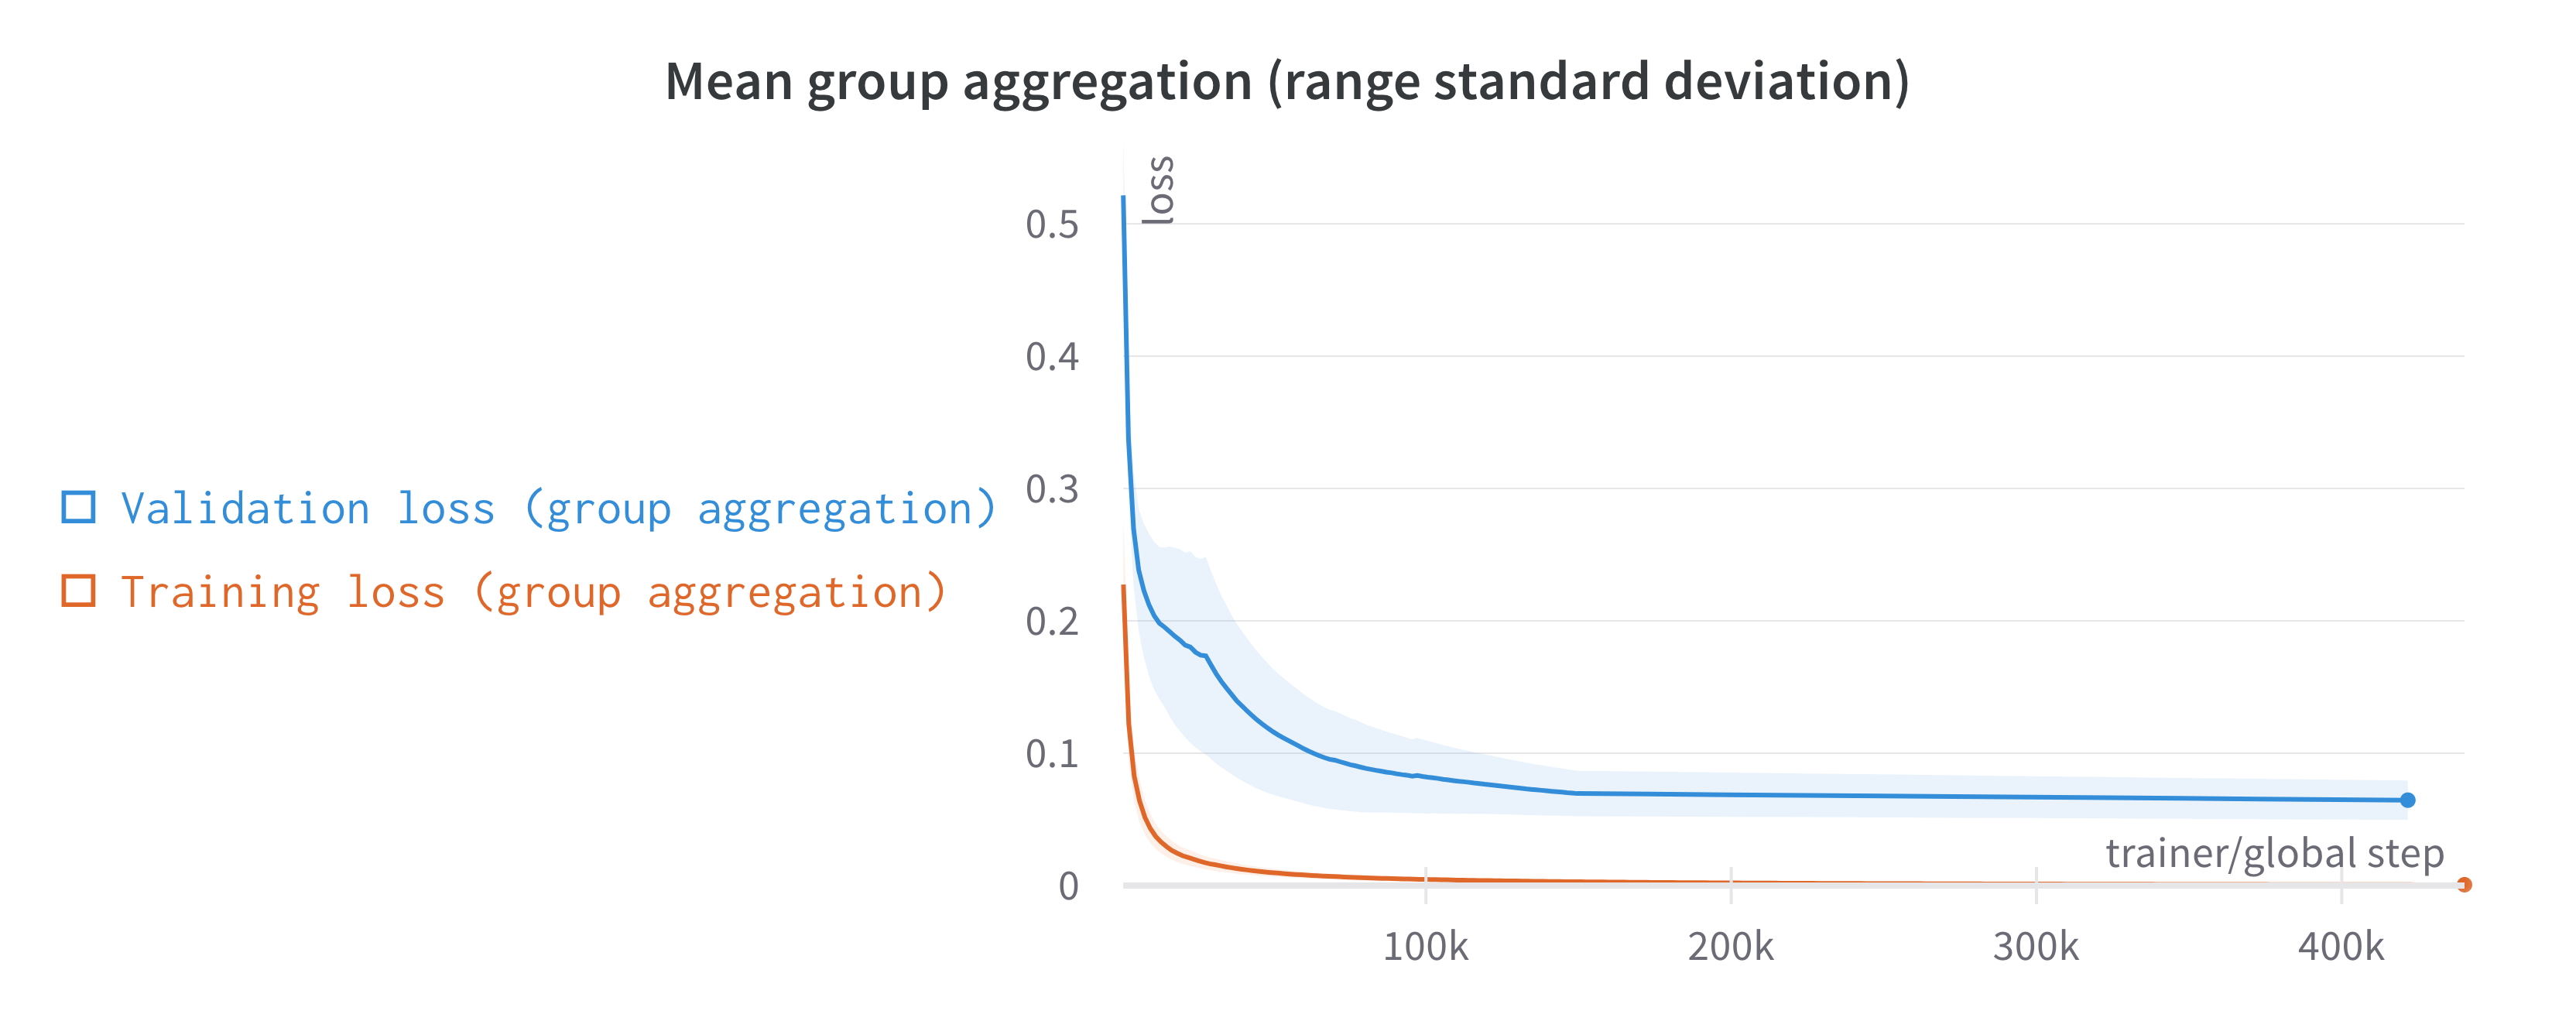
\includegraphics[width=\textwidth]{figures/images/Mean group aggregation.png}
    \caption{Caption}
    \label{fig:enter-label}
\end{figure}



\newpage


